\section{Perancangan Sistem}
Sistem yang dikembangkan menggunakan platform Java dengan model pemrograman berorientasi objek, untuk itu pemodelan sistem menggunakan bahasa UML \emph{(Unified Modelling Language)}. Adapun diagram UML yang digunakan untuk merepresentasikan sistem adalah \emph{usecase diagram, activity diagram} dan \emph{class diagram}.

\begin{figure}[hb]
    \centering
    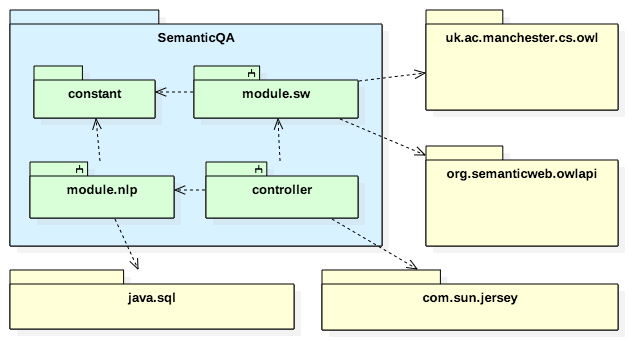
\includegraphics[width=1\textwidth]{bab_4/overview_package}
    \caption{Paket sistem \emph{question answering}}
    \label{fig:overview_package}
\end{figure}

Diagram \emph{usecase} digunakan untuk menunjukkan interaksi sistem dengan aktor atau pengguna, berapa jumlah aktor serta hak akses masing-masing aktor terhadap sistem. Sistem \emph{question answering} yang akan dibangun hanya memiliki satu buah layanan yaitu pencarian informasi kabupaten di Nusa Tenggara Barat, untuk itu sistem hanya melibatkan satu aktor tunggal yaitu pengguna yang akan memberikan pertanyaan kepada sistem seperti yang terlihat dalam Gambar \ref{fig:usecase_diagram}.

\begin{figure}[ht]
    \centering
    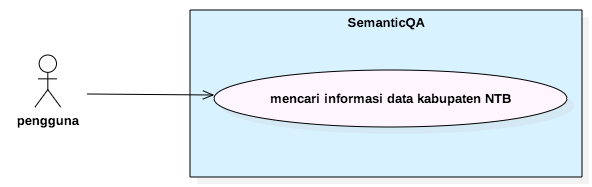
\includegraphics[width=0.8\textwidth]{bab_4/usecase_diagram2}
    \caption{Diagram \emph{usecase} sistem \emph{question answering}}
    \label{fig:usecase_diagram}
\end{figure}

Komponen-komponen penyusun server terdiri dari tiga buah paket utama seperti yang ditunjukkan dalam Gambar \ref{fig:overview_package}, yaitu \emph{controller, nlp} dan \emph{sw}. Sistem \emph{question answering} juga menggunakan \emph{library} pendukung pihak ketiga yaitu \emph{java sql connector} sebagai konektor basis data lexicon, \emph{jersey} untuk membentuk web service, \emph{Hermit reasoner, Sesame} serta \emph{OWL API} untuk penanganan ontologi.

Sistem \emph{question answering} melalui beberapa tahapan pemrosesan hingga menghasilkan jawaban, tahapan-tahapan yang dilakukan oleh sistem dapat dijelaskan dengan menggunakan diagram \emph{activity} seperti ditunjukkan dalam Gambar \ref{fig:activity_diagram}.

\begin{figure}[hb]
    \centering
    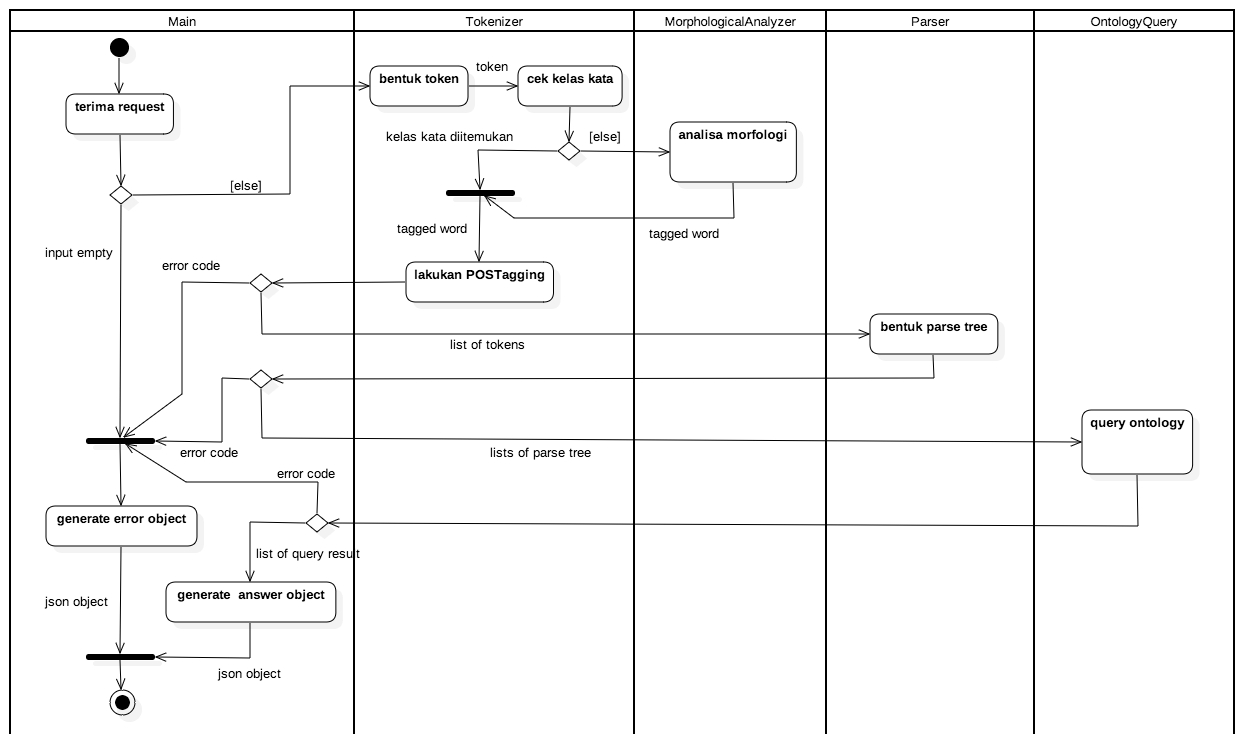
\includegraphics[width=1\textwidth]{bab_4/activity_diagram}
    \caption{\emph{activity diagram}}
    \label{fig:activity_diagram}
\end{figure}

\subsection{Paket \emph{controller}}
Paket \emph{controller} hanya terdiri dari satu buah kelas yaitu Main. Kelas ini terdiri dari tiga buah metode yaitu \emph{search(), query()} dan \emph{buildResponse()} seperti ditunjukkan dalam Gambar \ref{fig:sub_sistem_endpoint}. Metode \emph{search()} menerima masukan berupa string yang merupakan pertanyaan yang dikirimkan oleh \emph{client}, metode ini memiliki akses kenampakan public.

\begin{figure}[hb]
    \centering
    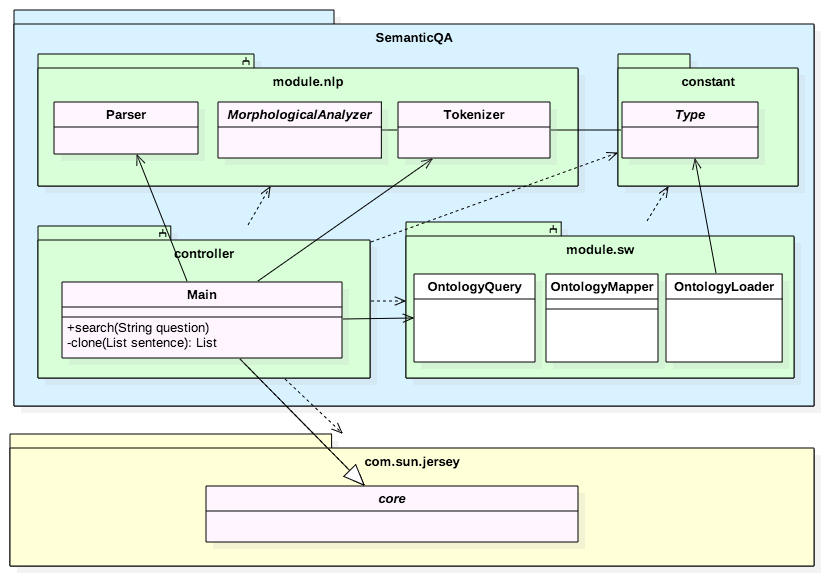
\includegraphics[width=1\textwidth]{bab_4/sub_sistem_endpoint}
    \caption{Struktur dan interaksi modul \emph{endpoint}} 
    \label{fig:sub_sistem_endpoint}
\end{figure}

Metode \emph{buildResponse()} berfungsi untuk membentuk objek JSON yang nantinya akan dikirimkan kepada klien sebagai respon. Adapun format objek JSON yang dihasilkan diperlihatkan dalam Gambar \ref{fig:json_response_object}.

Objek ``code'' berisi angka kode sesuai dengan kode standar yang digunakan oleh protokol HTTP, sedangkan objek ``message'' berisi string pesan sebagai penjelasan dari objek kode. Objek ``answer'' berisi objek yang terdiri dari ``text'' dan ``inferedFacts''. ``text'' berisi kalimat rangkuman jawaban atas pertanyaan yang diberikan sedangkan array ``inferedFacts'' berisi objek informasi hasil proses inferensi pertanyaan yang diberikan. Misalnya proses inferensi pertanyaan ``Siapa bupati kabupaten lombok timur ?'' menghasilkan menemukan fakta ``Fulan'' dan ``Lombok Timur'', maka array ``inferedFacts'' akan berisi properti-properti yang dimiliki oleh ``Fulan'' dan ``Lombok Timur''.

\begin{figure}[ht]
    \centering
    \begin{lstlisting}[language=XML,xleftmargin=0pt]
    {
        "code" : <code>,
        "message": <pesan_teks>,
        "answer": {
            "text":<teks rangkuman jawaban>,
            "inferedFacts":[
                <array objek hasil proses query dan reasoning>
            ]
        }
    }
\end{lstlisting}
    \caption{Rancangan respon objek JSON}
    \label{fig:json_response_object}
\end{figure}

Pertanyaan dikirimkan oleh \emph{client} dalam bentuk query parameter \emph{q}, parameter ini kemudian akan ditangkap dan diperiksa oleh metode \emph{search()}, jika query string berupa string kosong maka metode \emph{search()} akan langsung memanggil metode \emph{buildResponse()} dengan mengirimkan kode 204 yang mengindikasikan \emph{no content}. Jika query string dianggap valid maka metode \emph{search()} akan memulai proses pencarian dengan melakukan proses tokenisasi dengan melakukan proses instansiasi kelas Tokenizer dan memanggil metode \emph{tokenize()} dengan query parameter yang diterima sebelumnya sebagai parameter masukan. Apabila proses tokenisasi berhasil, maka selanjutnya metode \emph{search()} akan melakukan instansiasi kelas Parser dan memanggil metode \emph{parse()} dengan array list token sebagai masukan untuk membentuk pohon urai. Apabila proses pembentukan pohon urai gagal, dimana metode \emph{parse()} tidak menghasilkan pohon urai dan metode \emph{search()} akan memanggil metode \emph{buildRespone()} dengan mengirimkan kode 406 yang mengindikasikan pesan kesalahan \emph{not acceptable}.

Apabila proses pembentukan pohon urai berhasil, maka metode \emph{search()} akan melakukan instansiasi kelas OntologyQuery dan akan mengirimkan \emph{array list parse tree} yang sudah dibentuk. Kembalian hasil query ontologi berupa array list yang selanjutnya akan dikirimkan ke metode \emph{buildRespone()} untuk membentuk objek JSON yang selanjutnya akan dikirimkan kepada \emph{client} sebagai respon.

\subsection{Modul pemrosesan bahasa alami}
Modul pemrosesan bahasa alami terdiri dari tiga buah kelas seperti ditunjukkan dalam Gambar \ref{fig:sub_sistem_nlp} yaitu: Tokenizer, MorphologicalAnalyzer dan Parser. Kelas Tokenizer berfungsi untuk merubah query string yang dikirimkan oleh klien menjadi array list token kata yang telah diberi penanda kelas kata.

\begin{figure}[ht]
    \centering
    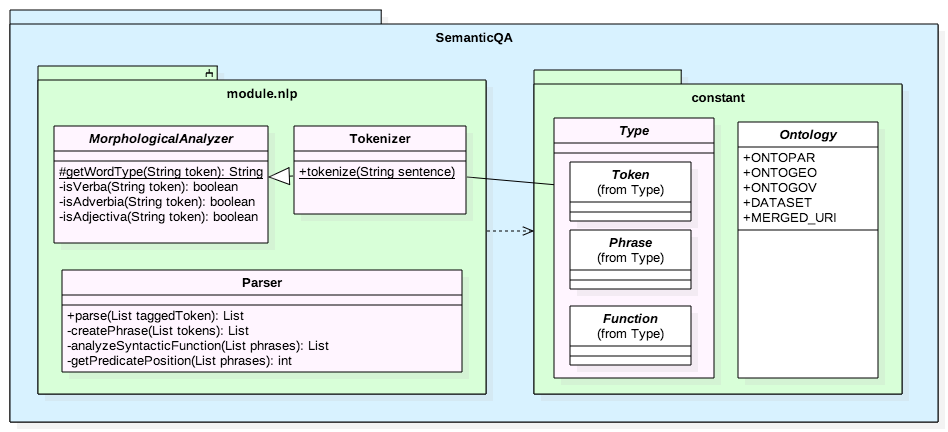
\includegraphics[width=1\textwidth]{bab_4/sub_sistem_nlp}
    \caption{Struktur modul pemrosesan bahasa alami} 
    \label{fig:sub_sistem_nlp}
\end{figure}


Pemrosesan bahasa alami diawali dengan pembentukan token serta pemberian \emph{POS-Tagging} pada masing-masing token kata untuk mengenali kelas katanya. Adapun diagram alir proses pembentukan token dan \emph{POS-Tagging} diperlihatkan pada Gambar \ref{fig:flowchart_proses_tokenisasi}.

\begin{figure}[ht]
    \centering
    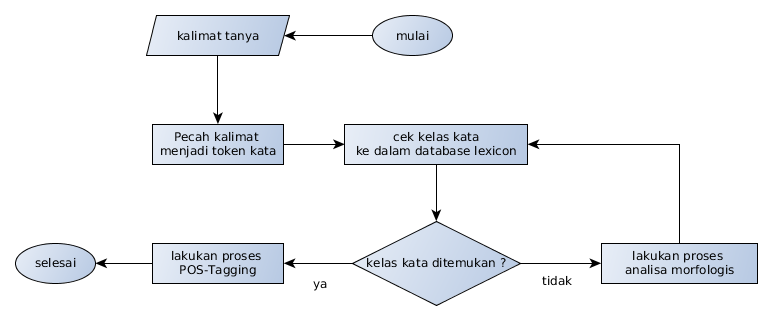
\includegraphics[width=1\textwidth]{bab_4/flowchart_proses_tokenisasi}
    \caption{Alur proses tokenisasi kalimat tanya}
    \label{fig:flowchart_proses_tokenisasi}
\end{figure}

Proses pengenalan kelas kata dilakukan dengan cara memeriksa kata yang bersangkutan ke dalam basis data \emph{lexicon}. Basis data \emph{lexicon} berupa basis data SQL yang terdiri dari satu buah tabel yang berisi kumpulan kata dasar bahasa Indonesia beserta dengan kelas katanya. Apabila kelas kata tidak ditemukan dalam tabel, maka proses dilanjutkan dengan menebak kelas kata dalam kelas \emph{MorphologicalAnalyzer}. Metode \emph{getWordType()} dalam kelas \emph{MorphologicalAnalyzer} akan menebak kelas kata dengan cara melakukan analisa bentuk morfologis kata yang bersangkutan berdasarkan aturan morfologi bahasa Indonesia yang dijelaskan oleh \citet{alwi}. Apabila semua aturan morfologis tidak terpenuhi, maka kata yang bersangkutan dianggap sebagai kata benda dan akan diberikan kelas kata Nomina (kata benda).

Proses selanjutnya adalah membangun pohon urai \emph{(parse tree)} dari token-token kata yang telah diberikan \emph{POS-Tangging}. Pembentukan \emph{parse tree} bertujuan untuk mengetahui fungsi sintaksis masing-masing frasa konstituen kalimat tanya. Alur proses pembentukan \emph{parse tree} diperlihatkan pada Gambar \ref{fig:flowchart_proses_parsing}. Data masukan proses pembentukan \emph{parse tree} adalah berupa array list token yang telah diberikan \emph{POS-Tagging}.

\begin{figure}[!ht]
    \centering
    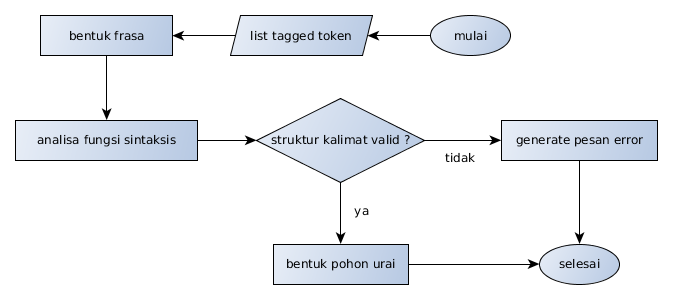
\includegraphics[width=.8\textwidth]{bab_4/flowchart_proses_parsing}
    \caption{Alur proses pembentukan \emph{parse tree}}
    \label{fig:flowchart_proses_parsing}
\end{figure}

Metode \emph{createPhrase()} dalam kelas Parser berfungsi untuk membentuk pohon urai awal yaitu pohon urai yang belum memiliki fungsi sintaksis frasa. Pohon urai yang telah dibentuk dalam metode \emph{createPhrase()} selanjutnya dikirimkan ke metode \emph{analyzeSyntacticFunction()} untuk dilakukan proses analisa dan penentuan fungsi sintaksis frasa yang terdapat di dalam pohon urai. Metode \emph{createPhrase()} menerima masukan berupa array list kata yang telah diberi kelas kata pada proses tokenisasi sedangkan metode \emph{analyzeSyntacticFunction()} menerima masukan berpa array list frasa. Pembentukan pohon urai dilakukan dengan menggunakan metode \emph{bottom-up} dimana proses pemeriksaan aturan-aturan bahasa dimulai dari konstituen kalimat yang kemudian dilanjutkan dengan frasa hingga membentuk kalimat utuh. Apabila selama proses terdapat aturan yang tidak terpenuhi, maka proses pembentukan pohon urai akan dihentikan dan pembentukan pohon urai dianggap gagal.

% Apabila proses pembentukan pohon urai berhasil, maka langkah selanjutnya adalah membangun 
% \begin{figure}[!ht]
%     \centering
%     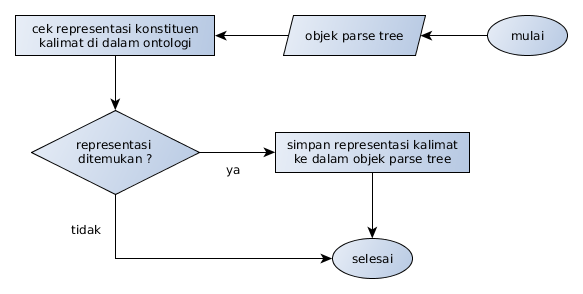
\includegraphics[width=.8\textwidth]{bab_4/flowchart_proses_ontology_mapper}
%     \caption{Alur proses \emph{mapping} konstituen kalimat ke dalam ontologi}
% \end{figure}


\subsection{Modul pemrosesan ontologi}
Modul pemrosesan ontologi merupakan modul utama yang terdri dari tiga buah kelas seperti yang ditunjuk\-kan dalam Gambar \ref{fig:sub_sistem_ontologi} masing-masing OntologyLoader, OntologyMapper dan OntologyQuery. 

\begin{figure}[hb]
    \centering
    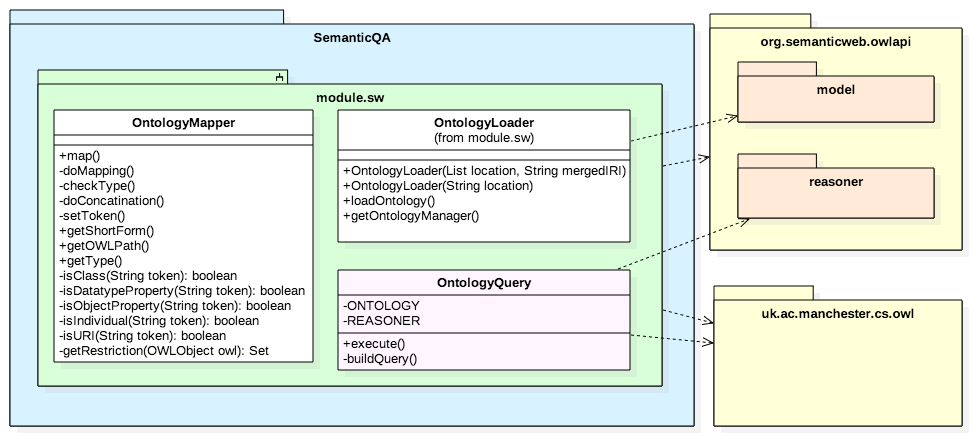
\includegraphics[width=1\textwidth]{bab_4/sub_sistem_ontologi}
    \caption{Struktur modul pemrosesan ontologi} 
    \label{fig:sub_sistem_ontologi}
\end{figure}

Modul pemrosesan ontologi menerima masukan data berupa \emph{prase tree} yang telah melalui proses \emph{ontology mapping} dimana proses ini akan memetakan konstituen-konstituen kalimat ke dalam ontologi. \emph{Parse tree} kemudian dianalisa untuk membentuk \emph{query} SPARQL-DL untuk selanjutnya diberikan kepada modul \emph{query engine} untuk dilakukan proses \emph{query} terhadap ontologi, proses \emph{query} juga melibatkan proses \emph{reasoning} untuk mendapatkan informasi-informasi yang bersifat eksplisit yang terdapat di dalam ontologi.

Apabila proses \emph{query} SPARQL-DL tidak berhasil atau objek hasil \emph{query} kosong, maka sistem akan membentuk objek pesan kesalahan, sedangkan apabila proses \emph{query} berhasil maka langkah selanjutnya adalah menganalisa individual ontologi hasil \emph{query}. Analisa dilakukan untuk menentukan apakah sistem perlu melakukan \emph{query} terhadap \emph{endpoint} DBPedia atau tidak. Adapun analisa yang dilakukan adalah memeriksa URI dari individual, apabila URI individual adalah merupakan URI yang berasal dari DBPedia maka sistem akan melakukan proses pembentukan query SPARQL dan sistem akan melakukan \emph{query} terhadap \emph{endpoint} DBPedia Indonesia. Langkah terakhir adalah menggabungkan data-data hasil \emph{query} terhadap \emph{endpoint} DBPedia Indonesia dengan data-data hasil query SPARQL-DL sebelumnya untuk dijadikan sebagai objek respon. Langkah pemrosesan ontologi diperlihatkan pada Gambar \ref{fig:flowchart_pemrosesan_ontologi}. 

\begin{figure}[ht]
    \centering
    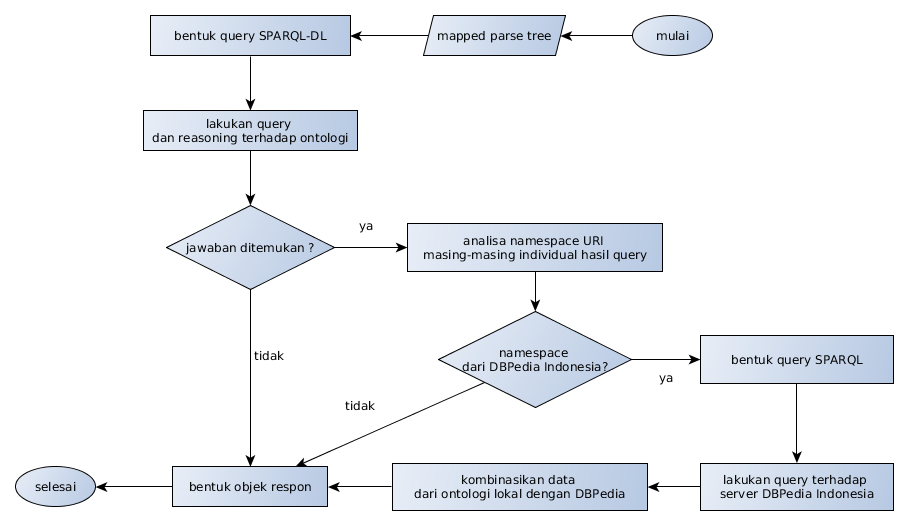
\includegraphics[width=1\textwidth]{bab_4/flowchart_proses_pemrosesan_ontologi}
    \caption{Alur proses query terhadap ontologi dan \emph{endpoint} DBPedia Indonesia}
    \label{fig:flowchart_pemrosesan_ontologi}
\end{figure}

Kelas OntologyMapper berfungsi untuk mencari representasi konstituen frasa di dalam ontologi. Proses awal pemetaan dilakukan melalui metode \emph{map()}, metode ini akan memanggil metode \emph{doMapping()} dengan mengirimkan pohon urai yang telah dibuat dalam kelas Parser. Proses pemetaan dilakukan secara rekursif hingga seluruh konstituen frasa yang terdapat di dalam pohon urai habis di proses. Konstituen frasa yang telah dicek akan disimpan ke dalam daftar token yang telah diproses dan akan disertakan pada iterasi selanjutnya. Daftar token yang telah diproses terebut nantinya akan digunakan untuk memeriksa kemungkinan objek ontologi yang berupa gabungan dua buah kata atau lebih, misalnya ``Lombok\_Timur''. Apabila gabungan dua buah konstituen kalimat atau lebih menemukan representasi objek ontologi, maka representasi yang baru juga akan turut disimpan sebagai konstituen baru dari kalimat sehingga konstituen frasa akan bertambah.

Kelas OntologyLoader berfungsi sebagai kelas yang menangani pemanggilan pemrosesan awal ontologi yaitu berupa proses \emph{loading} dan \emph{merging} tiga buah ontologi yang digunakan sebagai sumber basis pengetahuan. Sistem akan menggabungkan ketiga buah ontologi menjadi satu kesatuan, objek ontologi yang memiliki URI yang sama akan digabungkan menjadi satu, sehingga tidak terdapat objek ontologi ganda. Query SPARQL-DL memerlukan objek \emph{reasoner}, untuk itu OntologyLoader juga berfungsi untuk membuat objek \emph{reasoner}. 

Kelas OntologyQuery menangani proses pembentukan query serta pencarian data baik dari ontologi yang dibangun maupun dari DBPedia Indonesia. Proses diawali dengan memanggil metode \emph{execute()} dengan masukan berupa array list model Sentence yang telah melalui proses pemetaan. Metode \emph{execute()} selanjutnya akan memanggil metode \emph{buildQuery()} untuk membentuk query SPARQL-DL yang selanjutnya akan dieksekusi pada metode \emph{execute()}. Apabila objek hasil query berasal dari ontologi yang dibangun maka \emph{reasoner} akan melakukan pencarian persamaan objek yag didefinisikan oleh DBPedia. Apabila persamaan ditemukan maka akan dilakukan proses query SPARQL terhadap \emph{endpoint} DBPedia. Hasil query SPARQL-DL dan SPARQL selanjutnya akan dimasukkan ke dalam objek model QueryResultModel dan akan dikembalikan ke \emph{controller}.
